\chapter{Results} % Chapter title

\label{chapter:results} % For referencing the chapter elsewhere, use \ref{chapter:computational_neuro} 

\def \resultboxplot {0.8}
%----------------------------------------------------------------------------------------

\section{Multiple Query Optimization}
\label{chapter:results_mqo}

The non-ML circuit as well as the ML optimized one are run on the simulator as well as on real hardware. For this, the IBM Falcon r4L processor \code{ibmq\_bogota v1.6.37} is used. Each circuit runs 13 times, and the parity function referenced in the chapter \todo{add reference to parity explanation} is used for the ML optimized circuit as well as the non-ML circuit to allow for a direct comparison. For direct comparison, both the ML and non-ML circuit are evaluated using filtered and parity evaluation. The runs are made on a problem space $\left\mathcal{D}_{2\times2}|\right| =\ 300$, out of which 25\%, so 75 records, are taken and evaluated. These 75 records are the same used in the evaluation of the ML optimized circuit in chapter \ref{chapter:mqo_machine_learning}. The results are shown in figures \ref{figure:comparison_ml_noml_filtered_acc} - \ref{figure:ml_rhw_dist}.

\begin{figure}[!h]
    \centering
    \scalebox{\resultboxplot}{
        \includesvg{thesis/Appendices/comparison_ml_noml_circuit_filtered_acc.svg}
    }
    \caption{Direct comparison of the non-ML and ML circuits in terms of accuracy, once on the simulator (annotated with SIM) and once on real hardware (annotated with RHW). The accuracy is determined by the amount of best combinations the circuit evaluated to. The measured data is passed trough a filtered evaluation, which only considers valid combinational keys as results and not all. The ML circuit is not optimized with the filtered evaluation, but with the parity evaluation.}
    \label{figure:comparison_ml_noml_filtered_acc}
\end{figure}

\newpage

\begin{figure}[!h]
    \centering
    \scalebox{\resultboxplot}{
        \includesvg{thesis/Appendices/comparison_ml_noml_circuit_parity_acc.svg}
    }
    \caption{Direct comparison of the non-ML and ML circuits in terms of accuracy, once on the simulator (annotated with SIM) and once on real hardware (annotated with RHW). The accuracy is determined by the amount of best combinations the circuit evaluated to. The measured data is passed trough a parity evaluation, which takes the key with the highest probability.}
    \label{figure:comparison_ml_noml_parity_acc}
\end{figure}

The distance evaluation is done solely using the filtered evaluation method, as this results in the best accuracy, as shown in figures \ref{figure:comparison_ml_noml_filtered_acc} and \ref{figure:comparison_ml_noml_parity_acc}.

\begin{figure}[!h]
    \centering
    \scalebox{\resultboxplot}{
        \includesvg{thesis/Appendices/comparison_noml_sim_f_distance.svg}
    }
    \caption{Distance of the evaluated result to the best combination, where "Best" is the accumulation of how often the circuit evaluated onto the best combination, "2nd" being the second best combination etc. The non-ML circuit is run on the simulator and uses the filtered evaluation.}
    \label{figure:noml_sim_distance}
\end{figure}

\begin{figure}[!h]
    \centering
    \scalebox{\resultboxplot}{
        \includesvg{thesis/Appendices/comparison_noml_rhw_f_distance.svg}
    }
    \caption{Distance of the evaluated result to the best combination, where "Best" is the accumulation of how often the circuit evaluated onto the best combination, "2nd" being the second best combination etc. The non-ML circuit is run on real hardware and uses the filtered evaluation.}
    \label{figure:noml_rhw_dist}
\end{figure}

\begin{figure}[!h]
    \centering
    \scalebox{\resultboxplot}{
        \includesvg{thesis/Appendices/comparison_ml_sim_distanec.svg}
    }
    \caption{Distance of the evaluated result to the best combination, where "Best" is the accumulation of how often the circuit evaluated onto the best combination, "2nd" being the second best combination etc. The ML circuit is run on the simulator and uses the filtered evaluation.}
    \label{figure:ml_sim_distance}
\end{figure}



\begin{figure}[!h]
    \centering
    \scalebox{\resultboxplot}{
        \includesvg{thesis/Appendices/comparison_ml_rhw_distanec.svg}
    }
    \caption{Distance of the evaluated result to the best combination, where "Best" is the accumulation of how often the circuit evaluated onto the best combination, "2nd" being the second best combination etc. The ML circuit is run on real hardware and uses the filtered evaluation.}
    \label{figure:ml_rhw_dist}
\end{figure}

\newpage

To further evaluate both circuits with new, unseen data, the runs are executed again using a newly generated problem space $\left|\mathcal{D}_{2\times2}\right| =\ 1000$.

\begin{figure}[!h]
    \centering
    \scalebox{\resultboxplot}{
        \includesvg{thesis/Appendices/blind_run_noml_circuit_acc.svg}
    }
    \caption{Direct comparison of simulator and real hardware runs for the non-ML circuit in terms of accuracy, once on the simulator (annotated with SIM) and once on real hardware (annotated with RHW). The accuracy is determined by the amount of best combinations the circuit evaluated to. The measured data is passed trough a filtered evaluation, which only considers valid combinational keys as results and not all.}
    \label{figure:blind_run_noml_circuit_acc}
\end{figure}

\begin{figure}[!h]
    \centering
    \scalebox{\resultboxplot}{
        \includesvg{thesis/Appendices/blind_run_ml_circuit_f_acc.svg}
    }
    \caption{Direct comparison of simulator and real hardware runs for the ML circuit in terms of accuracy, once on the simulator (annotated with SIM) and once on real hardware (annotated with RHW). The accuracy is determined by the amount of best combinations the circuit evaluated to. The measured data is passed trough a filtered evaluation, which only considers valid combinational keys as results and not all.}
    \label{figure:blind_run_ml_circuit_f_acc}
\end{figure}

\begin{figure}[!h]
    \centering
    \scalebox{\resultboxplot}{
        \includesvg{thesis/Appendices/blind_run_ml_circuit_p_acc.svg}
    }
    \caption{Direct comparison of simulator and real hardware runs for the ML circuit in terms of accuracy, once on the simulator (annotated with SIM) and once on real hardware (annotated with RHW). The accuracy is determined by the amount of best combinations the circuit evaluated to. The measured data is passed trough a parity evaluation, which takes the key with the highest probability.}
    \label{figure:blind_run_ml_circuit_p_acc}
\end{figure}

\newpage

\subsection{Advanced Problem Spaces}
\label{chapter:results_advanced_problem_spaces}
As shown in chapter \ref{chapter:approach_and_methods}, the original problem generator was enhanced to allow for any combination of plans to be solved. As shown in chapter \ref{chapter:results_mqo}, the non-ML circuit achieves a better accuracy than its ML counterpart, whilst only losing marginal accuracy when running on real hardware. Due to this and time constraints, these \emph{dynamic} runs are done solely on the simulator using filtered evaluation and the non-ML circuit. The problem spaces are dynamically generated and always of size $\left|\mathcal{D}\right| =\ 5000$. Figure \ref{figure:overview_dynamic_problems} shows a comparison of all evaluated problem spaces $\mathcal{D}$, whilst figures \ref{figure:overview_dynamic_problems} to \ref{figure:bars_dist_3_3_3} show the distances of each run in detail.


\begin{figure}[!h]
    \centering
    \scalebox{\resultboxplot}{
        \includesvg{thesis/Appendices/comparison_accuracy_dynamic_problems.svg}
    }
    \caption{Comparison of different problem spaces $\left|\mathcal{D}\right| =\ 5000$ solved on the non-ML circuit. The accuracy reflects how often the evaluation led to the best combination. The x-axis is annotated with the plans per query.}
    \label{figure:overview_dynamic_problems}
\end{figure}

\begin{figure}[!h]
    \centering
    \scalebox{\resultboxplot}{
        \includesvg{thesis/Appendices/dynamic_problem_2_q_['2', '3']_p_dist.svg}
    }
    \caption{Distance of the evaluated result to the best combination, where "0" is the accumulation of how often the circuit evaluated onto the best combination, "1" being the second best combination etc. The non-ML circuit is run on the simulator and uses the filtered evaluation. The problem space $\mathcal{D}$ consists of 2 queries with one query having 2 and one 3 plans.}
    \label{figure:bars_dist_2_3}
\end{figure}

\begin{figure}[!h]
    \centering
    \scalebox{\resultboxplot}{
        \includesvg{thesis/Appendices/dynamic_problem_2_q_['3', '2']_p_dist.svg}
    }
    \caption{Distance of the evaluated result to the best combination, where "0" is the accumulation of how often the circuit evaluated onto the best combination, "1" being the second best combination etc. The non-ML circuit is run on the simulator and uses the filtered evaluation. The problem space $\mathcal{D}$ consists of 2 queries with one query having 3 and one 2 plans.}
    \label{figure:bars_dist_3_2}
\end{figure}

\begin{figure}[!h]
    \centering
    \scalebox{\resultboxplot}{
        \includesvg{thesis/Appendices/dynamic_problem_2_q_['3', '3']_p_dist.svg}
    }
    \caption{Distance of the evaluated result to the best combination, where "0" is the accumulation of how often the circuit evaluated onto the best combination, "1" being the second best combination etc. The non-ML circuit is run on the simulator and uses the filtered evaluation. The problem space $\mathcal{D}$ consists of 2 queries with both having 3 plans.}
    \label{figure:bars_dist_3_3}
\end{figure}

\begin{figure}[!ht]
    \centering
    \scalebox{\resultboxplot}{
        \includesvg{thesis/Appendices/dynamic_problem_2_q_['4', '2']_p_dist.svg}
    }
    \caption{Distance of the evaluated result to the best combination, where "0" is the accumulation of how often the circuit evaluated onto the best combination, "1" being the second best combination etc. The non-ML circuit is run on the simulator and uses the filtered evaluation. The problem space $\mathcal{D}$ consists of 2 queries with one query having 4 and one 2 plans.}
    \label{figure:bars_dist_4_2}
\end{figure}

\begin{figure}[!h]
    \centering
    \scalebox{\resultboxplot}{
        \includesvg{thesis/Appendices/dynamic_problem_2_q_['4', '3']_p_dist.svg}
    }
    \caption{Distance of the evaluated result to the best combination, where "0" is the accumulation of how often the circuit evaluated onto the best combination, "1" being the second best combination etc. The non-ML circuit is run on the simulator and uses the filtered evaluation. The problem space $\mathcal{D}$ consists of 2 queries with one query having 4 and one 3 plans.}
    \label{figure:bars_dist_4_3}
\end{figure}

\begin{figure}[!h]
    \centering
    \scalebox{\resultboxplot}{
        \includesvg{thesis/Appendices/dynamic_problem_2_q_['4', '4']_p_dist.svg}
    }
    \caption{Distance of the evaluated result to the best combination, where "0" is the accumulation of how often the circuit evaluated onto the best combination, "1" being the second best combination etc. The non-ML circuit is run on the simulator and uses the filtered evaluation. The problem space $\mathcal{D}$ consists of 2 queries with both having 4 plans.}
    \label{figure:bars_dist_4_4}
\end{figure}

\begin{figure}[!h]
    \centering
    \scalebox{\resultboxplot}{
        \includesvg{thesis/Appendices/dynamic_problem_3_q_['2', '2', '2']_p_dist.svg}
    }
    \caption{Distance of the evaluated result to the best combination, where "0" is the accumulation of how often the circuit evaluated onto the best combination, "1" being the second best combination etc. The non-ML circuit is run on the simulator and uses the filtered evaluation. The problem space $\mathcal{D}$ consists of 3 queries with each having 2 plans.}
    \label{figure:bars_dist_2_2_2}
\end{figure}

\begin{figure}[!h]
    \centering
    \scalebox{\resultboxplot}{
        \includesvg{thesis/Appendices/dynamic_problem_3_q_['2', '3', '2']_p_dist.svg}
    }
    \caption{Distance of the evaluated result to the best combination, where "0" is the accumulation of how often the circuit evaluated onto the best combination, "1" being the second best combination etc. The non-ML circuit is run on the simulator and uses the filtered evaluation. The problem space $\mathcal{D}$ consists of 3 queries with two having 2 plans and one 3 plans.}
    \label{figure:bars_dist_2_3_2}
\end{figure}

\begin{figure}[!h]
    \centering
    \scalebox{\resultboxplot}{
        \includesvg{thesis/Appendices/dynamic_problem_3_q_['3', '2', '3']_p_dist.svg}
    }
    \caption{Distance of the evaluated result to the best combination, where "0" is the accumulation of how often the circuit evaluated onto the best combination, "1" being the second best combination etc. The non-ML circuit is run on the simulator and uses the filtered evaluation. The problem space $\mathcal{D}$ consists of 3 queries with two having 3 plans and one 2 plans.}
    \label{figure:bars_dist_3_2_3}
\end{figure}

\begin{figure}[!h]
    \centering
    \scalebox{\resultboxplot}{
        \includesvg{thesis/Appendices/dynamic_problem_3_q_['3', '3', '3']_p_dist.svg}
    }
    \caption{Distance of the evaluated result to the best combination, where "0" is the accumulation of how often the circuit evaluated onto the best combination, "1" being the second best combination etc. The non-ML circuit is run on the simulator and uses the filtered evaluation. The problem space $\mathcal{D}$ consists of 3 queries with each having 3 plans.}
    \label{figure:bars_dist_3_3_3}
\end{figure}

\begin{sidewaysfigure}
    \centering
    \scalebox{1.0}{
\Qcircuit @C=1.0em @R=0.2em @!R { \\
                \nghost{{q}_{0} :  } & \lstick{{q}_{0} :  } & \gate{\mathrm{H}} \barrier[0em]{4} & \qw & \gate{\mathrm{R_Y}\,(\mathrm{-1.0*c0})} \barrier[0em]{4} & \qw & \ctrl{3} & \ctrl{4} & \qw & \qw & \qw & \qw \barrier[0em]{4} & \qw & \gate{\mathrm{R_X}\,(\frac{\pi}{4})} \barrier[0em]{4} & \qw & \qw & \qw\\
                \nghost{{q}_{1} :  } & \lstick{{q}_{1} :  } & \gate{\mathrm{H}} & \qw & \gate{\mathrm{R_Y}\,(\mathrm{-1.0*c1})} & \qw & \qw & \qw & \ctrl{2} & \ctrl{3} & \qw & \qw & \qw & \gate{\mathrm{R_X}\,(\frac{\pi}{4})} & \qw & \qw & \qw\\
                \nghost{{q}_{2} :  } & \lstick{{q}_{2} :  } & \gate{\mathrm{H}} & \qw & \gate{\mathrm{R_Y}\,(\mathrm{-1.0*c2})} & \qw & \qw & \qw & \qw & \qw & \ctrl{1} & \ctrl{2} & \qw & \gate{\mathrm{R_X}\,(\frac{\pi}{4})} & \qw & \qw & \qw\\
                \nghost{{q}_{3} :  } & \lstick{{q}_{3} :  } & \gate{\mathrm{H}} & \qw & \gate{\mathrm{R_Y}\,(\mathrm{-1.0*c3})} & \qw & \gate{\mathrm{R_Z}\,(\mathrm{s03})} & \qw & \gate{\mathrm{R_Z}\,(\mathrm{s13})} & \qw & \gate{\mathrm{R_Z}\,(\mathrm{s23})} & \qw & \qw & \gate{\mathrm{R_X}\,(\frac{\pi}{4})} & \qw & \qw & \qw\\
                \nghost{{q}_{4} :  } & \lstick{{q}_{4} :  } & \gate{\mathrm{H}} & \qw & \gate{\mathrm{R_Y}\,(\mathrm{-1.0*c4})} & \qw & \qw & \gate{\mathrm{R_Z}\,(\mathrm{s04})} & \qw & \gate{\mathrm{R_Z}\,(\mathrm{s14})} & \qw & \gate{\mathrm{R_Z}\,(\mathrm{s24})} & \qw & \gate{\mathrm{R_X}\,(\frac{\pi}{4})} & \qw & \qw & \qw\\
\\ }}
    \caption{Non-ML circuit dynamically generated for the problem space $\mathcal{D}$ with 2 queries, where one has 3 plans and the other 2 plans. This circuit evaluated and produces the results shown in figure \ref{figure:bars_dist_3_2}}
    \label{circuit:noml_dyn_problem}
\end{sidewaysfigure}

\newpage

\section{Quantum Neural Network}
\label{chapter:results_qnn}
All of the datasets mentioned in \ref{subsection:qnn_datasets_and_acqusition} have been trained, then evaluated on the remote general-purpose simulator \textit{ibmq\_qasm\_simulator} and on a real quantum system. The real quantum system named \textit{ibmq\_manila} uses the \code{Falcon} processor family in revision \code{r5.11} and with segment \code{L}.

\begin{itemize}
    \item \textbf{Family:} refers to the chip architecture. 
    \item \textbf{Revisions:} are design variants within a given family. 
    \item \textbf{Segment:} differentiates processors comprising different sub-sections of a larger chip.
\end{itemize}


\subsection{Evaluation On Simulator}
For evaluation we chose the weights from the best training run having the highest accuracy for each VQC and dataset. 

\textbf{Simulator:} General-purpose simulator \textit{ibmq\_qasm\_simulator}\footnote{\url{https://quantum-computing.ibm.com/services/docs/services/manage/simulator/#qasm}}.

\begin{table}[!h]
	\centering
	        
	\begin{tabular}{p{0.12\textwidth}p{0.15\textwidth}|p{0.13\textwidth}p{0.13\textwidth}p{0.13\textwidth}p{0.13\textwidth}}
		\hline 
		\textbf{Dataset}        & \textbf{VQC} & \textbf{COBYLA} & \textbf{SPSA}  & \textbf{AMSGR.} & \textbf{BFGS} \\
		\hline 
		\multirow{6}{*}{\textbf{Adhoc}}  & q\_circuit\_01 & 0.600  & 0.665 & 0.660   & 0.720 \\
		                        & q\_circuit\_02 & 0.700  & 0.795 & 0.650   & \underline{0.800} \\
		                        & q\_circuit\_03 & 0.700  & 0.705 & 0.660   & 0.650 \\
		                        & q\_circuit\_04 & 0.705 & 0.650 & 0.645   & 0.650 \\
		                        & q\_circuit\_05 & 0.565 & 0.690 & 0.65   & 0.715 \\
		\cline{2-6} 
		                        & \textbf{Average} & 0.654  & 0.701 & 0.653  & \textbf{0.707} \\
		\hline 
		\multirow{6}{*}{\textbf{Custom}} & q\_circuit\_01 & 0.515  & 0.550 & 0.700   & 0.630 \\
		                        & q\_circuit\_02 & 0.690  & 0.550 & 0.500   & 0.605 \\
		                        & q\_circuit\_03 & 0.700  & 0.645 & 0.500   & 0.700 \\
		                        & q\_circuit\_04 & 0.590  & 0.535 & 0.550  & 0.520 \\
		                        & q\_circuit\_05 & 0.505  & 0.65 & 0.615   & \underline{0.740} \\
		\cline{2-6} 
		                        & \textbf{Average}      & 0.600 & 0.586 & 0.573   & \textbf{0.639} \\
		\hline 
		\multirow{6}{*}{\textbf{Iris}}   & q\_circuit\_01 & 1.00  & 1.00 & 1.00   & 1.00 \\
		                        & q\_circuit\_02 & 1.00  & 1.00 & 1.00   & 1.00 \\
		                        & q\_circuit\_03 & 1.00  & 1.00 & 1.00   & 1.00 \\
		                        & q\_circuit\_04 & 1.00  & 0.885 & 0.950   & 1.00 \\
		                        & q\_circuit\_05 & 1.00  & 1.00 & 1.00   & 1.00 \\
		\cline{2-6} 
		                        & \textbf{Average}      & \textbf{1.00}  & 0.977 & 0.990   & \textbf{1.00} \\
		\hline 
		\multirow{6}{*}{\textbf{Rain}}   & q\_circuit\_01 & 0.745  & 0.665 & 0.650   & 0.730 \\
		                        & q\_circuit\_02 & 0.625  & 0.665 & 0.785   & 0.695 \\
		                        & q\_circuit\_03 & 0.580 & 0.800 & 0.800  & 0.720 \\
		                        & q\_circuit\_04 & 0.395  & 0.545 & \underline{0.825}   & 0.570 \\
		                        & q\_circuit\_05 & 0.620 & 0.620 & 0.615   & 0.685 \\
		\cline{2-6} 
		                        & \textbf{Average}      & 0.593  & 0.659 & \textbf{0.735}   & 0.680 \\
		\hline 
		\multirow{6}{*}{\textbf{Vlds}}   & q\_circuit\_01 & 0.845  & 0.820 & 0.800   & 0.800 \\
		                        & q\_circuit\_02 & 0.770  & 0.730 & 0.780   & 0.650 \\
		                        & q\_circuit\_03 & 0.795  & 0.760 & 0.750   & 0.790 \\
		                        & q\_circuit\_04 & 0.805  & 0.525 & 0.750   & \underline{0.925} \\
		                        & q\_circuit\_05 & 0.795  & 0.600 & 0.900   & 0.690 \\
		\cline{2-6} 
		                        & \textbf{Average}      & \textbf{0.802}  & 0.687 & 0.796   & 0.771 \\
		\hline
	\end{tabular}
	\caption{Comparison of accuracy for the optimizers COBYLA, SPSA, AMSGRAD (Adam) and BFGS over and average of 10 runs using two VQC layers for the quantum simulator training runs and binary datasets.}
	\label{table:accuracy_comparison_binary_dataset_and_optimizers_training_runs}
\end{table}


\subsection{Evaluation On Real Hardware}
Quantum system: \textit{ibmq\_manila} IBM Quantum Falcon\footnote{\url{https://quantum-computing.ibm.com/services/docs/services/manage/systems/processors#falcon}} Processors.

\begin{table}[!h]
	\centering
	        
	\begin{tabular}{p{0.12\textwidth}p{0.15\textwidth}|p{0.13\textwidth}p{0.13\textwidth}p{0.13\textwidth}p{0.13\textwidth}}
		\hline 
		\textbf{Dataset}        & \textbf{VQC} & \textbf{COBYLA} & \textbf{SPSA}  & \textbf{AMSGR.} & \textbf{BFGS} \\
		\hline 
		\multirow{6}{*}{\textbf{Adhoc}}  & q\_circuit\_01  & 0.610  & 0.645 & 0.650    & 0.715 \\
		                        & q\_circuit\_02 & \underline{0.745}  & \underline{0.745} & 0.665    & 0.715 \\
		                        & q\_circuit\_03 & 0.675  & 0.695 & 0.665    & 0.715 \\
		                        & q\_circuit\_04 & 0.650  & 0.650 & 0.655    & 0.65 \\
		                        & q\_circuit\_05 & 0.605  & 0.680 & 0.635    & 0.715 \\
		\cline{2-6} 
		                        & \textbf{Average} & 0.657  & 0.683 & 0.654    & \textbf{0.702} \\
		\hline 
		\multirow{6}{*}{\textbf{Custom}} & q\_circuit\_01  & 0.555  & 0.600 & 0.660    & 0.625 \\
		                        & q\_circuit\_02  & 0.655  & 0.575 & 0.500    & 0.620 \\
		                        & q\_circuit\_03  & 0.7  & 0.610 & 0.500    & 0.640 \\
		                        & q\_circuit\_04  & 0.57  & 0.515 & 0.550    & 0.500 \\
		                        & q\_circuit\_05  & 0.45  & 0.625 & 0.620    & \underline{0.750} \\
		\cline{2-6} 
		                        & \textbf{Average} & 0.586  & 0.585 & 0.566    & \textbf{0.627} \\
		\hline 
		\multirow{6}{*}{\textbf{Iris}}   & q\_circuit\_01 & 1.00  & 1.00 & 1.00    & 1.00 \\
		                        & q\_circuit\_02 & 1.00  & 0.865 & 1.00    & 1.00 \\
		                        & q\_circuit\_03 & 1.00  & 1.00 & 1.00    & 1.00 \\
		                        & q\_circuit\_04 & 1.00  & 0.885 & 0.955    & 0.805 \\
		                        & q\_circuit\_05 & 0.880  & 0.985 & 1.00    & 1.00 \\
		\cline{2-6} 
		                        & \textbf{Average} & 0.976  & 0.947 & \textbf{0.991}    & 0.961 \\
		\hline 
		\multirow{6}{*}{\textbf{Rain}}   & q\_circuit\_01 & 0.495  & 0.600 & 0.71 0  & 0.665 \\
		                        & q\_circuit\_02 & 0.710  & 0.635 & 0.715    & 0.665 \\
		                        & q\_circuit\_03 & 0.595  & \underline{0.790} & 0.745    & 0.550 \\
		                        & q\_circuit\_04 & 0.440  & 0.495 & 0.775    & 0.555 \\
		                        & q\_circuit\_05 & 0.650  & 0.470 & 0.640   & 0.620 \\
		\cline{2-6} 
		                        & \textbf{Average} & 0.578  & 0.598 & \textbf{0.717}    & 0.611 \\
		\hline 
		\multirow{6}{*}{\textbf{Vlds}}   & q\_circuit\_01 & 0.855  & 0.770 & 0.615    & 0.710 \\
		                        & q\_circuit\_02 & 0.705  & 0.885 & 0.740    & 0.635 \\
		                        & q\_circuit\_03 & 0.725  & 0.765 & 0.705    & 0.870 \\
		                        & q\_circuit\_04 & 0.81  & 0.485 & 0.750    & \underline{0.950} \\
		                        & q\_circuit\_05 & 0.755  & 0.615 & 0.745    & 0.735 \\
		\cline{2-6} 
		                        & \textbf{Average} & 0.770  & 0.704 & 0.711    & \textbf{0.780} \\
		\hline
	\end{tabular}
	\caption{Comparison of accuracy for the optimizers COBYLA, SPSA, AMSGRAD (Adam) and BFGS over and average of 10 runs using two VQC layers - bound to the weights of the highest scoring trainings run - for the quantum computer evaluation runs and binary datasets.}
	\label{table:accuracy_comparison_binary_dataset_and_optimizers_evaluation_runs}
\end{table}

\subsection{Comparison}


\begin{table}[!h]
	\centering
	\begin{tabular}{rccc}
		\hline 
		\thead{Dataset} & \thead{QNN (Quantum Simulator)} & \thead{QNN (Quantum Computer)} \\
		\hline 
		Iris    & 1.00     & 1.00  \\
		Rain    & 0.825    & 0.790 \\
		Vlds    & 0.925    & 0.950 \\
		Custom  & 0.74     & 0.750 \\
		Adhoc   & 0.800    & 0.745 \\
		\hline
		\textbf{Average}  & \textbf{0.858} & \textbf{0.847}  \\
		\hline
	\end{tabular}
	\caption{Comparison of the QNN accuracy on a quantum simulator as well as on a real quantum computer. The table shows the accuracy of the best approach for each of the VQCs and optimizer types using the binary datasets.}
	\label{table:comparison_binary_datasets_accuracy}
\end{table}

\begin{figure}[!ht]
    \centering
    \\[-3ex]
    \begin{subfigure}{1.0\textwidth}
        \centering
        \subcaption{Iris}
        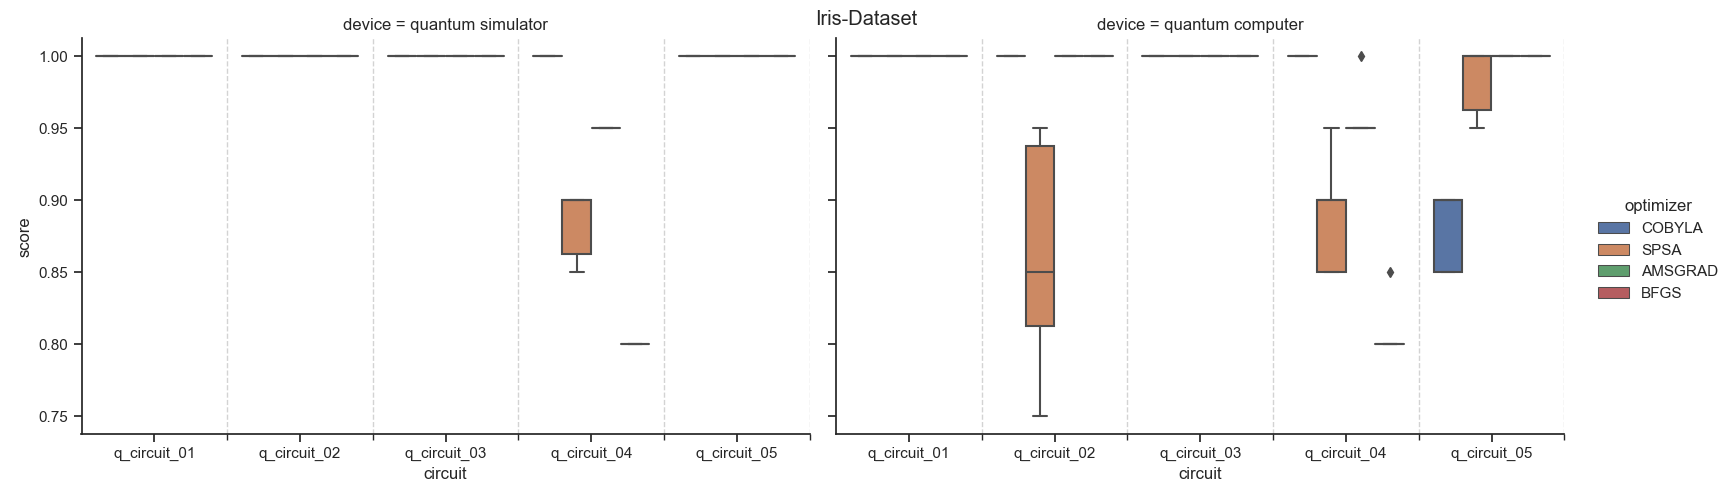
\includegraphics[width=1.0\linewidth]{thesis/Figures/qnn/boxplots/100_iris.png} 
        \label{subfigure:accuracy_comparison_boxplots_iris_dataset1}
    \end{subfigure}
    \\[-3ex]
    \begin{subfigure}{1.0\textwidth}
        \centering
        \subcaption{Rain}
        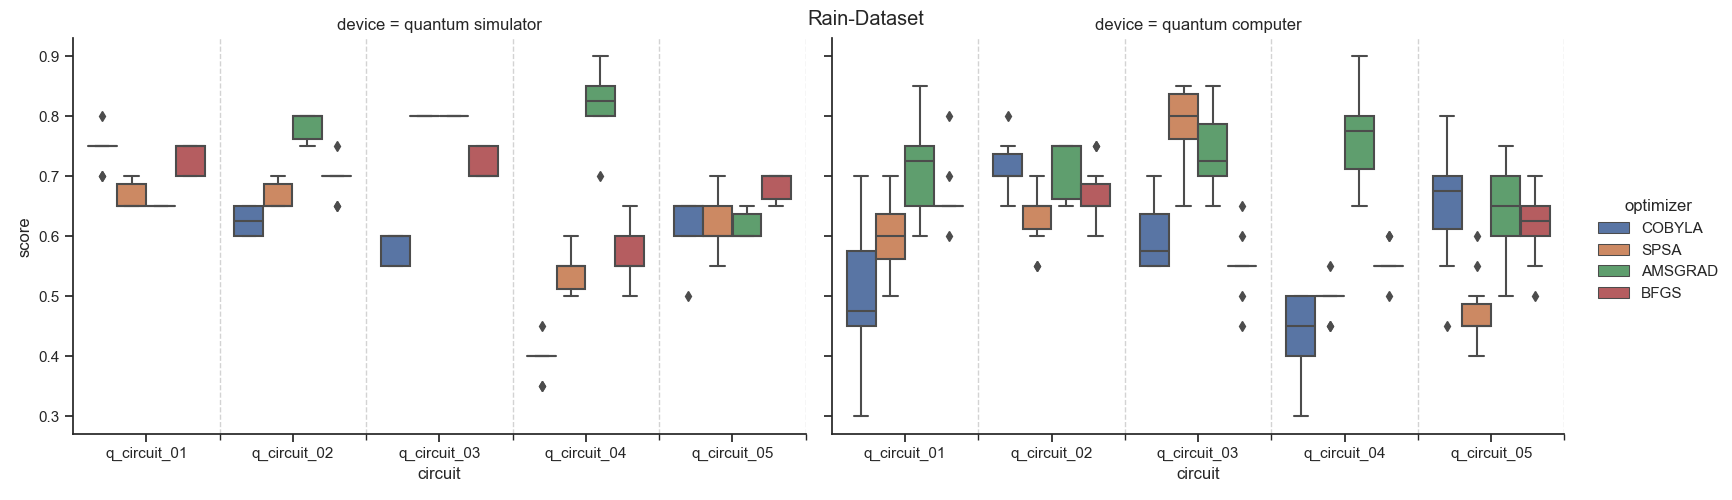
\includegraphics[width=1.0\linewidth]{thesis/Figures/qnn/boxplots/100_rain.png} 
        \label{subfigure:accuracy_comparison_boxplots_rain_dataset1}
    \end{subfigure}
    \\[-3ex]
    \begin{subfigure}{1.0\textwidth}
        \centering
        \subcaption{Vlds}
        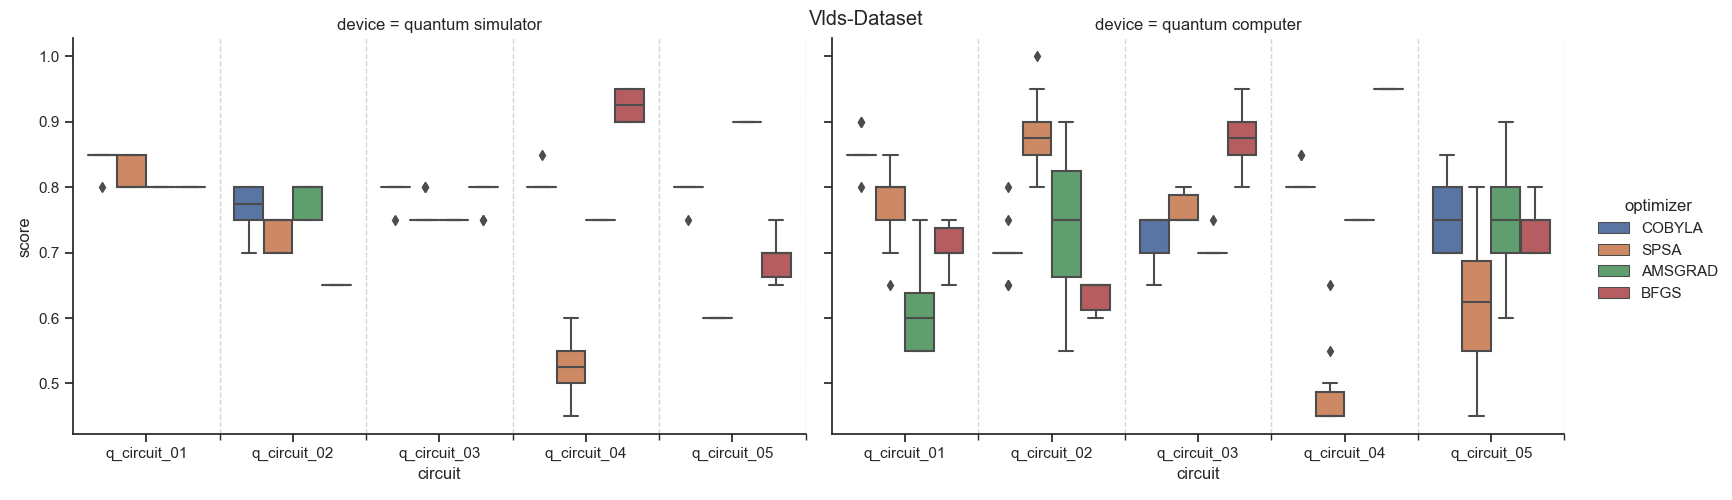
\includegraphics[width=1.0\linewidth]{thesis/Figures/qnn/boxplots/100_vlds.png} 
        \label{subfigure:accuracy_comparison_boxplots_vlds_dataset1}
    \end{subfigure}
    \\[-3ex]
    \begin{subfigure}{1.0\textwidth}
        \centering
        \subcaption{Custom}
        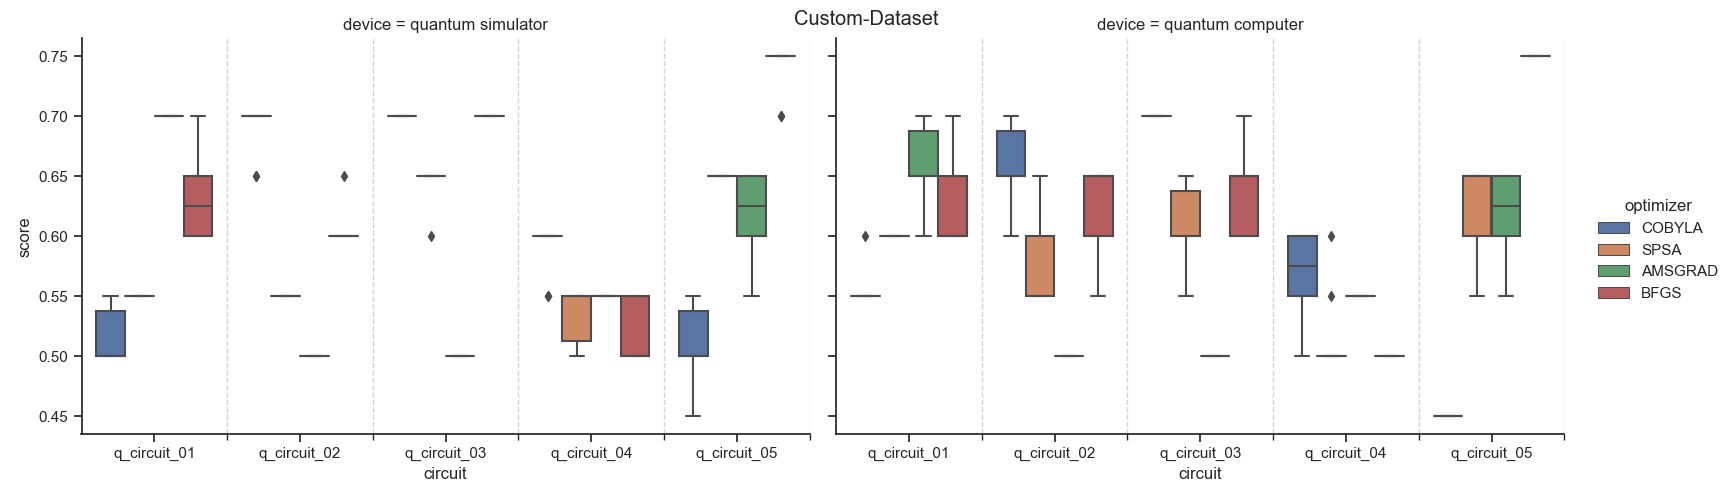
\includegraphics[width=1.0\linewidth]{thesis/Figures/qnn/boxplots/100_custom.png}
        \label{subfigure:accuracy_comparison_boxplots_custom_dataset1}
    \end{subfigure}
    \\[-3ex]
    \begin{subfigure}{1.0\textwidth}
        \centering
        \subcaption{Adhoc}
        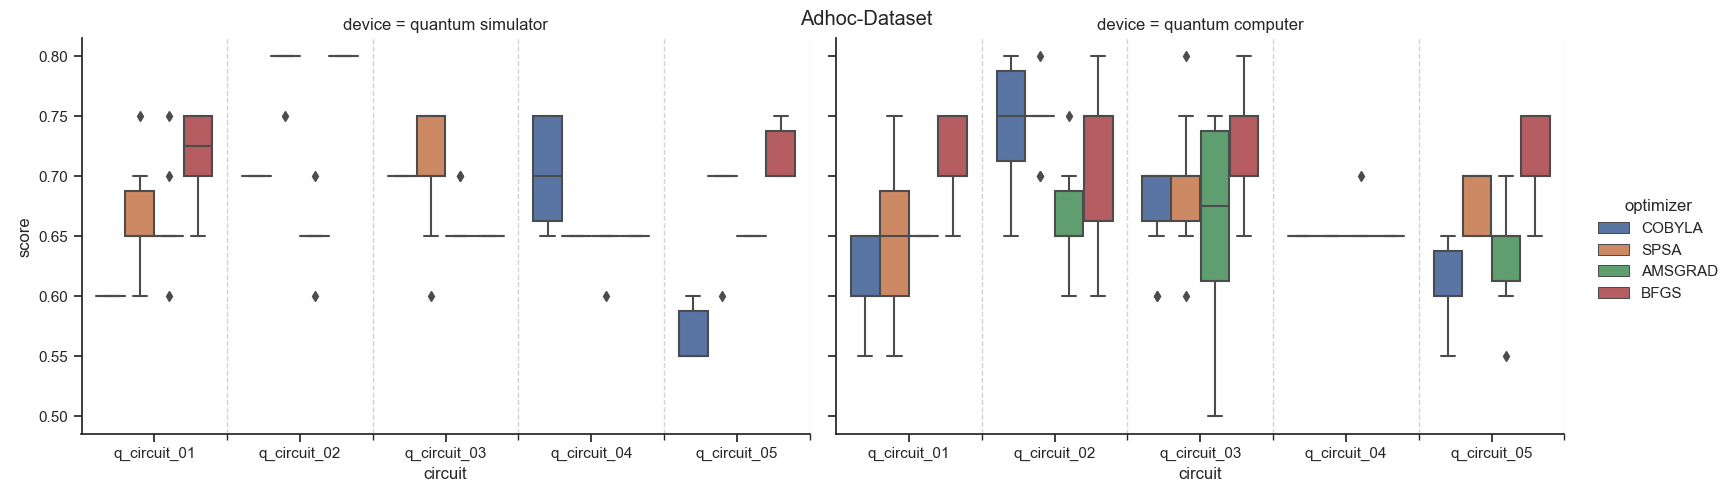
\includegraphics[width=1.0\linewidth]{thesis/Figures/qnn/boxplots/100_adhoc.png}
        \label{subfigure:accuracy_comparison_boxplots_adhoc_dataset1}
    \end{subfigure}
    \\[-3ex]
    \caption{Average accuracy comparison of 10 runs on the quantum simulator and computer for all binary datasets, circuits and optimizers.}
    \label{figure:accuracy_comparison_boxplots_binary_datasets}
\end{figure}


\clearpage